\apendice{Tecnologias}
\label{ap:tecnologias}

A arquitetura do software foi desenvolvida em três partes: servidor, banco de dados e cliente. Tanto o lado cliente (\textit{frontend}) como o lado servidor(\textit{backend})
utilizam a linguagem Javascript.
Na parte do servidor, ou \textit{server-side}, foram utilizados NodeJS, Express e Mongoose. No lado do cliente foram utilizadas as seguintes tecnologias:
HTML, CSS, Javascript (EcmaScript 6), AngularJS e o Dynagraph. O banco de dados MongoDB foi utilizado como suporte a leitura inicial dos dados.


\section{Servidor}
O \textit{backend} foi utilizado para manipular o banco de dados e transformar as informações na estrutura de dados do Dynagraph para permitir sua análise no \textit{frontend}.
O Node.js é uma plataforma de desenvolvimento para executar código Javascript no \textit{server side} sobre o motor JavaScript do Google Chrome para facilmente construir aplicações de rede rápidas e escaláveis. Uma das maiores vantagens do Node.js é que ele usa um modelo de I/O direcionada a evento não bloqueante que o torna leve e eficiente, ideal para aplicações em tempo real com troca intensa de dados através de dispositivos distribuídos.

O Express.js é um framework JavaScript que facilita a criação de aplicativos web utilizando o Node.js e fornece um conjunto robusto de recursos para aplicativos web e móvel. Com vários métodos utilitários HTTP e \textit{middleware} disponíveis para criar uma API robusta, rápida e fácil. 

Mongoose é uma biblioteca do Nodejs que proporciona uma solução baseada em esquemas para modelar os dados da sua aplicação. Ele possui sistema de conversão de tipos, validação, criação de consultas e \textit{hooks} para lógica de negócios. Mongoose fornece um mapeamento de objetos do MongoDB similar ao ORM (Object Relational Mapping), ou ODM (Object Data Mapping) no caso do Mongoose. Isso significa que o Mongoose traduz os dados do banco de dados para objetos JavaScript para que possam ser utilizados por sua aplicação.

\section{Banco de dados}

MongoDB é um dos mais populares de banco de dados NoSQL. O mesmo é open-source e escrito em C++.
MongoDB é um banco de dados orientado a documentos que armazena dados em documentos JSON com esquema dinâmico. Isso significa que você pode armazenar seus registros sem se preocupar com a estrutura de dados, como o número de campos ou tipos de campos para armazenar valores. Os documentos do MongoDB são semelhantes aos objetos JSON.

\section{Cliente}

%HTML
O HTML é uma Linguagem de Marcação de Hipertexto (\textit{Hypertext Markup Language}) utilizada para criar páginas web. Ele descreve a estrutura das páginas web usando marcadores (\textit{markup}). Os seus elementos são construídos em blocos de páginas HTML e são representados por \textit{tags}. Tags de HTML marcam partes de conteúdo, como "cabeçalho" (\textit{heading}), "parágrafo" (\textit{paragraph}), "tabela" (\textit{table}) e assim por diante. Os navegadores não exibem as tags HTML, mas as usam para renderizar o conteúdo da página \cite{html}.

%CSS
 Junto ao HTML temos o CSS (\textit{Cascading Style Sheets}), que é uma linguagem que descreve o estilo (\textit{style}) de um documento HTML. Além disso, ele descreve como os elementos HTML devem ser exibidos. Uma das vantagens em utilizar o CSS é controlar o \textit{layout} de múltiplas páginas web ao mesmo tempo. Ele é projetado para permitir a separação de apresentação e conteúdo, incluindo layout, cores e fontes. Essa separação pode melhorar a acessibilidade de conteúdo, fornecer mais flexibilidade e controle na especificação de características de apresentação e reduzir a complexidade e a repetição no conteúdo estrutural \cite{css}.

%Javascript
O JavaScript é uma linguagem de programação interpretada, frequentemente abreviado como JS, de alto nível, caracterizada como dinâmica, fracamente tipada, baseada em protótipos, de tipagem fraca.
O ECMAScript é uma linguagem de programação baseada em scripts, padronizada pela Ecma International na especificação ECMA-262. A linguagem é bastante usada em tecnologias para Internet, sendo esta base para a criação do JavaScript. A versão utilizada do ECMAScript para esta pesquisa foi a ECMAScript 6 ou ECMAScript2015 \cite{ecma2015}.

%JSON
Outro recurso associado ao \textit{frontend} é o JSON (\textit{JavaScript Object Notation}), que é um formato “leve” para troca de informações. Ele é baseado em um subconjunto da linguagem de programação JavaScript  \cite{json} e também em dois tipos de estruturas: Coleção de pares chave/valor e lista ordenada de valores. As coleções de chave e valor são equivalentes a record, struct, dictionary, hash e map nas linguagens. As listas são equivalentes a array, vector ou list.
Um objeto é um conjunto não ordenado de pares nome/valor. Um objeto começa com { (chave esquerda) e termina com } (chave direita). Cada nome é seguido por : (dois pontos) e os pares nome/valor são separados por , (vírgula).

%AngularJS
O Editor de Características foi incorporado ao Dynagraph após a sua conclusão, e o seu desenvolvimento foi realizado utilizando principalmente o framework AngularJS \cite{angularjs}.
Este permite construir aplicações web dinâmicas e estender a sintaxe do HTML, e com isso simplifica o código e permite uma estrutura componentizada. A ligação de dados e a injeção de dependência do AngularJS eliminam grande parte do código que seria necessário escrever.
Seu principal padrão arquitetural é o MVC (\textit{Model View Controller}):
\begin{itemize}
	\item Modelo (\textit{Model}): são as propriedades de um escopo; escopos são anexados ao DOM onde as propriedades do escopo são acessadas por meio de ligações.
	\item Visão (\textit{View}): O \textit{template} (HTML com ligações de dados) que é renderizado na Visão.
	\item Controlador (\textit{Controller}): é a classe que contém a lógica de negócios por trás do aplicativo.
\end{itemize}


Dynagraph (HTML 5)

\section{Arquitetura do Software}
A princípio o MongoDB foi utilizado para armazenar os dados salvos do \cite{simda}, a respeito da dengue e chikungunya. O cliente requisita os dados do servidor, que por sua vez processa as informações, seguindo a estrutura de dados do Dynagraph. Em seguida, esses dados processados são passados para a aplicação no cliente. Com os dados exibidos no browser podemos editá-los, gerar agrupamentos e finalmente salvar as informações em um arquivo no formato JSON.

\begin{figure}[h]
	\centering	
	\Caption{\label{fig:arqsoft} Arquitetura do Softwate}	
	\UECEfig{}{
		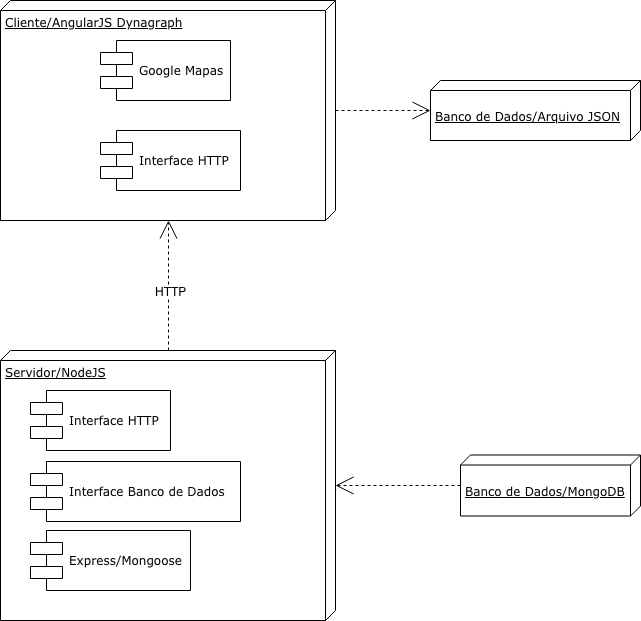
\includegraphics[width=14cm]{figuras/apendice/dissertacaoArquitetura.png}
	}{
		\Fonte{Elaborado pelo autor}
	}
\end{figure}
\FloatBarrier

\section{Ferramentas e Materiais}
O desenvolvimento do trabalho foi realizado a partir dos seguintes equipamentos e materiais:
\begin{itemize}
	\item Macbook Pro 13" modelo 2015 / macOS High Sierra 10.13.2:
	\subitem Processador Intel Core i5 2.7 GHz;
	\subitem Memória de 8GB 1867 MHzs DDR3;
	\subitem HD SSD 128GB;
	\item Ambiente de desenvolvimento Webstorm;
	\item Navegador de internet Google Chrome 63.0.3239.132.
	\item Controle de versão Git (Software e dissertação);
	\item \LaTeX para produção da dissertação;
	\item Portal de periódicos CAPES;
\end{itemize}